\documentclass{article}
\usepackage{graphicx}
\usepackage[margin=1.5cm]{geometry}
\usepackage{amsmath}

\begin{document}

\title{Introduction to Vectors: Displacement and Velocity}
\author{Prof. Jordan C. Hanson}

\maketitle

\begin{abstract}
The purpose of this group activity is to practice problem-solving with vectors.  \textit{Displacement} is a vector that represents translational motion.  This is distinct from \textit{distance}, which is a scalar quantity representing the total amount of length an object has traversed.  \textit{Velocity} is displacement divided by time duration.  In this activity, we will attempt to navigate a dogfight between F-18 aircraft in the movie Top Gun: Maverick.
\end{abstract}

\section{The Problem Statement - Maverick}

\textit{Top Gun: Maverick} is a film detailing a complex mission given to 5th generation fighter pilots who must revert to older F18 aircraft for technical reasons.  They undergo training with a reknowned and infamous Navy pilot nicknamed Maverick (Tom Cruise).  In one scene, Maverick is attacking two pairs of his students by first flying at an altitude low enough to be within radar clutter.  Maverick ascends beneath them, and passes right between the pair of craft, blowing their minds and engines.

Let a two-dimensional \textit{x-z} coordinate system describe the space in which the aircraft maneuver.  The appropriate unit of distance for the area is the kilometer, or 1000.0 m.  The initial position of the pilots in training is $\vec{x}_{i,t} = (0.0, 2.1)$ km.  The initial position for Maverick is $\vec{x}_{i,m} = (0.0, 0.1)$ km.  The initial velocity of all craft is $\vec{v}_{i,s} = (v_x,0.0)$ km/hr.  The situation is depicted in Fig. \ref{fig:hunt1}.

\begin{figure}[hb]
\centering
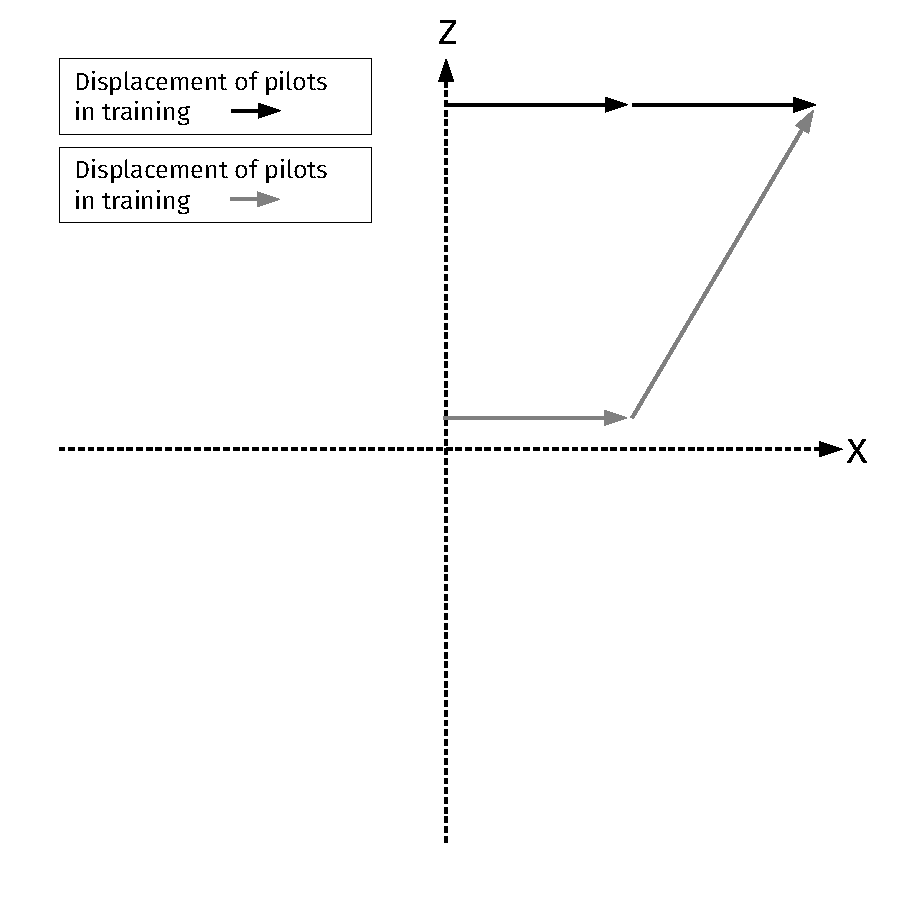
\includegraphics[width=0.5\textwidth,trim=0cm 6cm 0cm 0cm,clip=true]{TheHuntForRedOctober1.pdf}
\caption{\label{fig:hunt1}  In the first stage of the exercise, Maverick flies parallel to his targets, but below them.  In the second stage, he ascends in a way that allows him to blow by them at a point he must calculate in his head.}
\end{figure}

\section{Initial Displacements}

\textit{Displacement} is formally defined as the difference between the final position and the initial position:

\begin{equation}
\Delta \vec{x} = \vec{x}_f - \vec{x}_i
\end{equation}

If $v_x = 500$ km/hr, give the displacement vectors of the craft after 30 seconds: \\ \vspace{1cm}

$\Delta \vec{x}_t = (?,?)~~~~~~~~~~\Delta \vec{x}_m = (?,?)$

\section{Final Displacement of the Pilots in Training}

If the velocity $\vec{v}_t = (v_x,0)$ km/hr of the pilots in training remains constant, calculate their location after another 10 seconds passes.  \\ \vspace{1cm}

$\vec{x}_t = (?,?)$

\section{Vector Velocity}

In that same 10 seconds, Maverick changes course and meets the other pilots at their location.  We will now calculate the displacement required to get his craft to the location of the other craft.  Use final location minus initial location to obtain displacement:

\begin{equation}
\Delta \vec{x}_m = \vec{x}_{m,f} - \vec{x}_{m,i}
\end{equation}

The \textbf{vector velocity} of Maverick is given by 

\begin{equation}
\vec{v}_m = \frac{\Delta \vec{x}_m}{\Delta t}
\end{equation}

Let $\Delta t = 10$ seconds.  What velocity does Maverick need to reach his targets in 10 seconds? \\ \vspace{2cm}

$\vec{v}_m = (?,?)$ \\ \vspace{2cm}

Let's compute the percent increase in the \textit{speed} of Maverick.  The speed is the magnitude of the velocity.  Using Pythagorean theorem, compute the magnitude of $\vec{v}_m$, and compare it to the magnitude of his velocity in the beginning of the exercise.  What is the percent increase?

\end{document}
